\begin{figure}[t]
\centering
% Vector drawing generated by tools/figures/maintenance.py; rerun it after changing the figure.
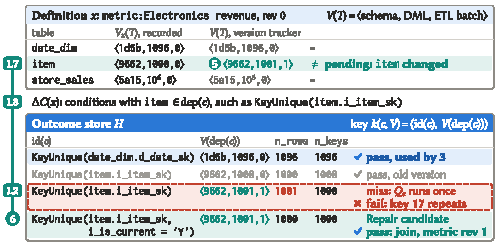
\includegraphics[width=\columnwidth]{figures/maintenance}%
\caption{\bt{Lookup after the \code{item} load (steps 5--6; L$n$ marks line $n$ of Algorithm~\ref{alg:maintenance}). Only \code{item}'s stamp changed, so only the \code{item} key check reruns, once, at its new key; the \code{date\_dim} outcome still serves three definitions.}{\code{item} 载入后的查找（步骤 5--6；L$n$ 指算法~\ref{alg:maintenance} 第 $n$ 行）。只有 \code{item} 的版本戳变化，因此只有 \code{item} 键检查在新键上重跑一次；\code{date\_dim} 的检查结果仍服务三个定义。}}
\label{fig:maintenance}
\Description{Top: the stamps of definition x, metric:Electronics revenue, revision 0, where a stamp V(T) is (schema fingerprint, DML count, ETL batch). For each table the recorded stamp V_x(T) is next to the version tracker's current stamp V(T): date_dim (1d5b, 1096, 0) equals (1d5b, 1096, 0); store_sales (5a15, 10^6, 0) equals itself; item (9662, 1000, 0) differs from (9662, 1001, 1), produced by the ETL load (step 5), so the definition is pending (tag L7). Tag L8: Delta C(x) is the set of conditions whose dep(c) contains item, such as KeyUnique(item.i_item_sk). Bottom: the outcome store H with key k(c, V) = (id(c), V(dep(c))) and columns n_rows and n_keys. Row 1, highlighted: KeyUnique(date_dim.d_date_sk) at (1d5b, 1096, 0), 1096 rows over 1096 keys, pass, used by 3. Row 2, grey: KeyUnique(item.i_item_sk) at (9662, 1000, 0), 1000 over 1000, pass, old version. Row 3, red dashed, tag L2: KeyUnique(item.i_item_sk) at (9662, 1001, 1), miss, Q_c runs once, 1001 rows over 1000 keys, fail: key 17 repeats. Row 4, step 6: KeyUnique(item.i_item_sk, i_is_current = 'Y') at (9662, 1001, 1), the Repair candidate, 1000 over 1000, pass, join and metric revision 1. A vertical line connects tags L7, L8, L2 and step 6 down the left edge.}
\end{figure}
